\label{sect:mgt}

\eucommentary{Will get help from Orsay's grant services}

\eucommentary{Describe the organizational structure and the decision-making
(including a list of milestones (table 3.2a)).\\
Explain why the organizational structure and decision-making mechanisms are
 appropriate to the complexity and scale of the project.\\
Describe, where relevant, how effective innovation management will be
addressed in the management structure and work plan.\\
Describe any critical risks, relating to project implementation, that
the stated project's objectives may not be achieved. Detail any risk
mitigation measures. Please provide a table with critical risks
identified and mitigating actions (table 3.2b).}


\begin{tabular}{|m{.4\textwidth}|c|m{.5\textwidth}|}
  \hline
  Risk & Level & Mitigation measures\\\hline

  Recruiting qualified personnel & Medium &
  whenever possible, we coordinate with currently running projects to rehire
  personnel with well known high level competences\\\hline
slmhnlnhfnhs&hsfhs&ghshsh\\\hline

\end{tabular}


%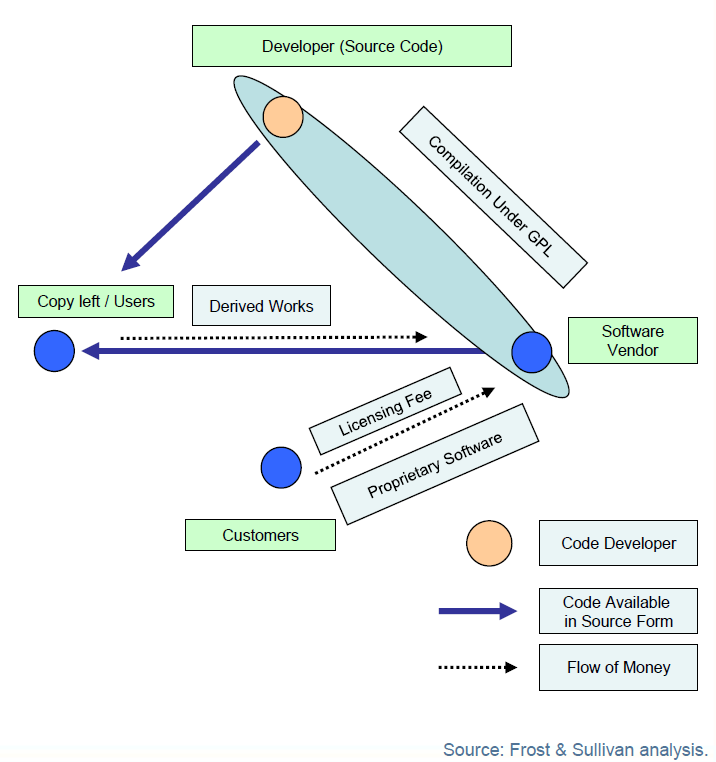
\includegraphics[width=.94\textwidth]{Pictures/Impact-img1.png}


\TODO{An open source architecture allows risk sharing: collaborating
  in the early stages of research could help an early detection, and,
  by consequence, reducing risks.}

\TODO{But: since Open Source softwares are freely accessible, security
  and privacy issues are a concern. Anytime a resource is shared,
  there is greater risk of unauthorised access and contaminated data.
  Providers must demonstrate security solutions, which should include
  physical security controlling access to the facility and protection
  of user data from corruption and cyber attacks.}

